

\subsection{Experiment on 10 graphs}

\subsubsection{Degree distribution}

Show in Figure \ref{fig:as-skitter_degree_dist} to  \ref{fig:soc-Slashdot0811_degree_dist}.
\\
The degree distributions in most of graphs follow power law. We found that there were spikes in p2p-Gnutella31 outdegree and degree distribution. The reason for the spike may be because of default peer number of setting in p2p software. Besides p2p graph, there were little spikes in email-Enron and soc-Slashdot0811. 

\begin{figure}
\subfloat[In-Degree Distribution\label{fig:as-skitter_indegree}]
  {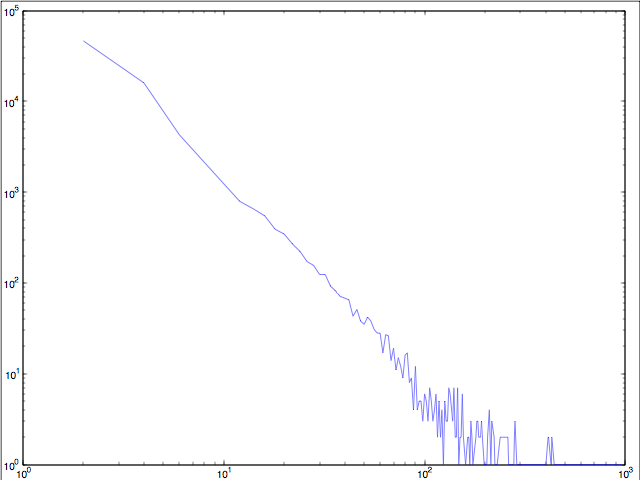
\includegraphics[width=.3\linewidth]{FIG/as-skitter.75000-indd.png}}\hfill
\subfloat[Out-Degree Distribution\label{fig:as-skitter_outdegree}]
  {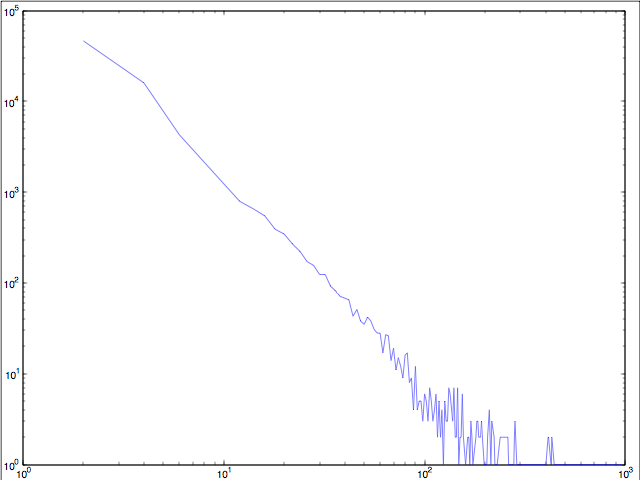
\includegraphics[width=.3\linewidth]{FIG/as-skitter.75000-outdd.png}}\hfill
\subfloat[Degree Distribution\label{fig:as-skitter_degree}]
  {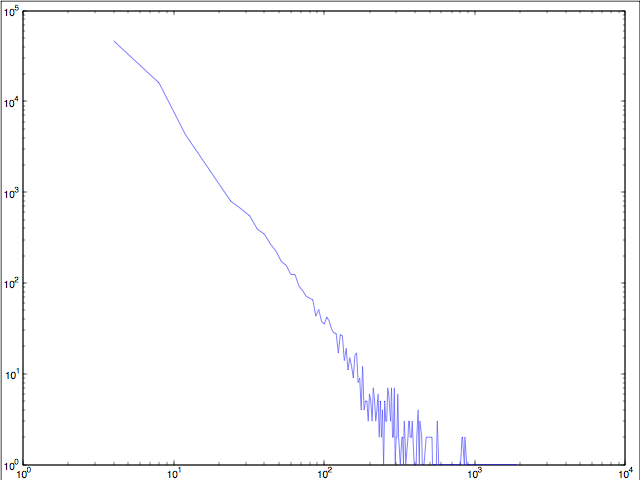
\includegraphics[width=.3\linewidth]{FIG/as-skitter.75000-dd.png}}
\caption{Degree Distributions of as-skitter\label{fig:as-skitter_degree_dist}}
\end{figure}
\begin{figure}
\subfloat[In-Degree Distribution\label{fig:ca-AstroPh_indegree}]
  {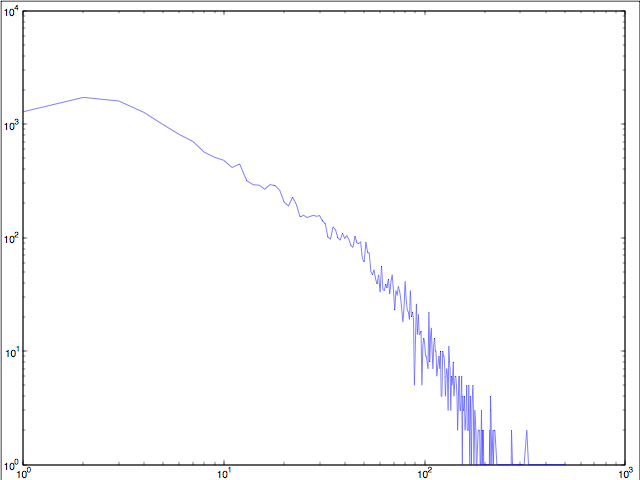
\includegraphics[width=.3\linewidth]{FIG/ca-AstroPh-indd.png}}\hfill
\subfloat[Out-Degree Distribution\label{fig:ca-AstroPh_outdegree}]
  {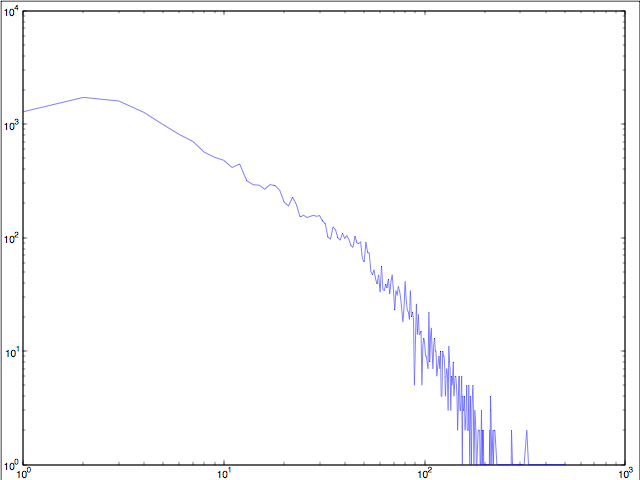
\includegraphics[width=.3\linewidth]{FIG/ca-AstroPh-outdd.png}}\hfill
\subfloat[Degree Distribution\label{fig:ca-AstroPh_degree}]
  {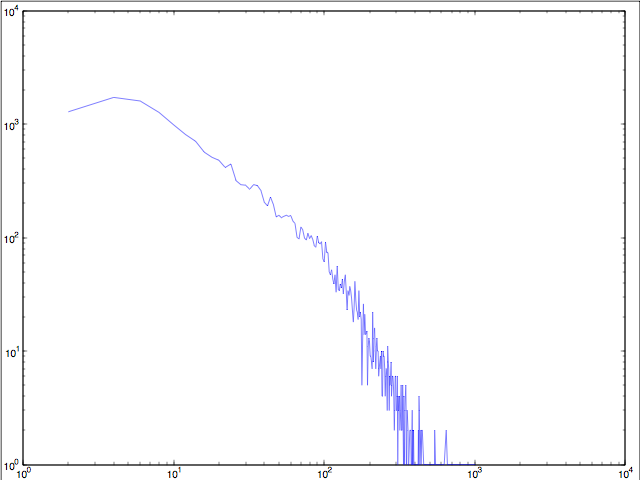
\includegraphics[width=.3\linewidth]{FIG/ca-AstroPh-dd.png}}
\caption{Degree Distributions of a-AstroPh\label{fig:ca-AstroPh_degree_dist}}
\end{figure}
\begin{figure}
\subfloat[In-Degree Distribution\label{fig:cit-HepPh_indegree}]
  {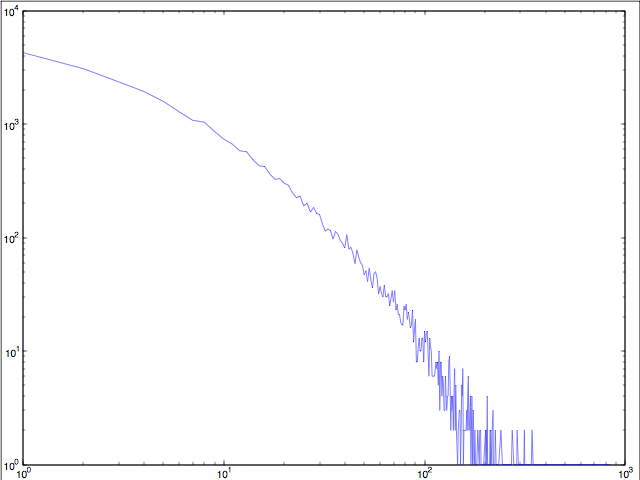
\includegraphics[width=.3\linewidth]{FIG/cit-HepPh-indd.png}}\hfill
\subfloat[Out-Degree Distribution\label{fig:cit-HepPh_outdegree}]
  {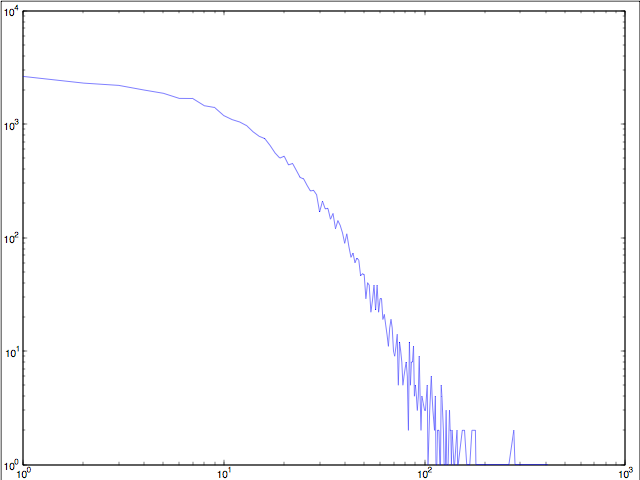
\includegraphics[width=.3\linewidth]{FIG/cit-HepPh-outdd.png}}\hfill
\subfloat[Degree Distribution\label{fig:cit-HepPh_degree}]
  {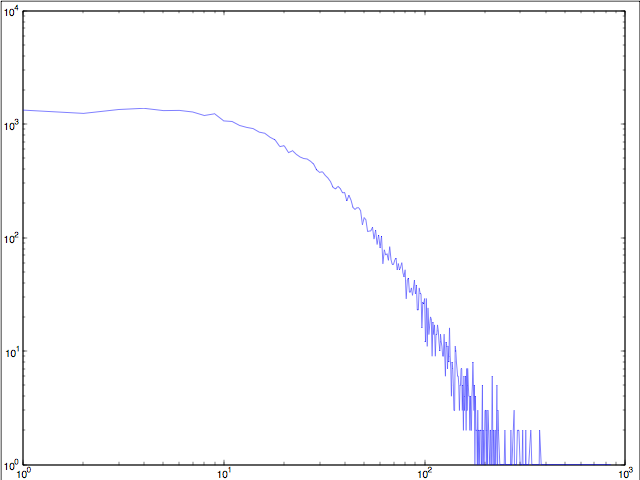
\includegraphics[width=.3\linewidth]{FIG/cit-HepPh-dd.png}}
\caption{Degree Distributions of cit-HepPh\label{fig:cit-HepPh_degree_dist}}
\end{figure}
\begin{figure}
\subfloat[In-Degree Distribution\label{fig:cit-HepTh_indegree}]
  {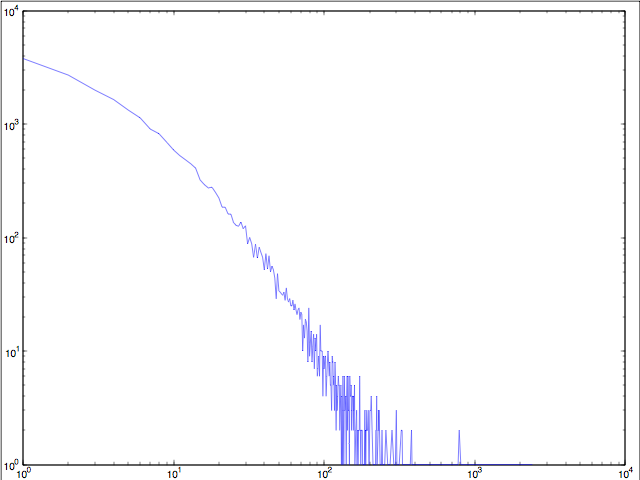
\includegraphics[width=.3\linewidth]{FIG/cit-HepTh-indd.png}}\hfill
\subfloat[Out-Degree Distribution\label{fig:cit-HepTh_outdegree}]
  {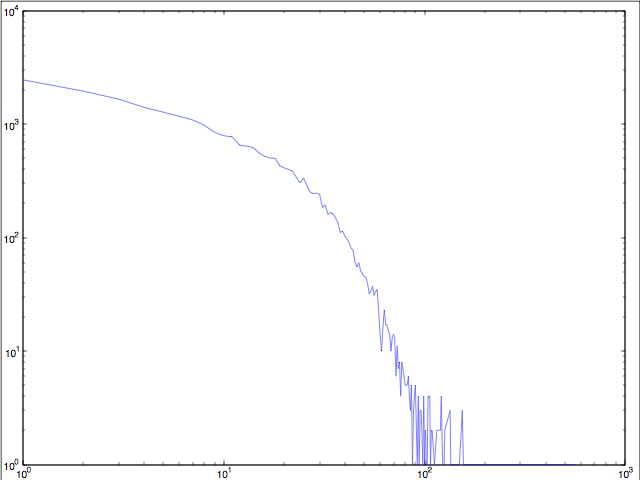
\includegraphics[width=.3\linewidth]{FIG/cit-HepTh-outdd.png}}\hfill
\subfloat[Degree Distribution\label{fig:cit-HepTh_degree}]
  {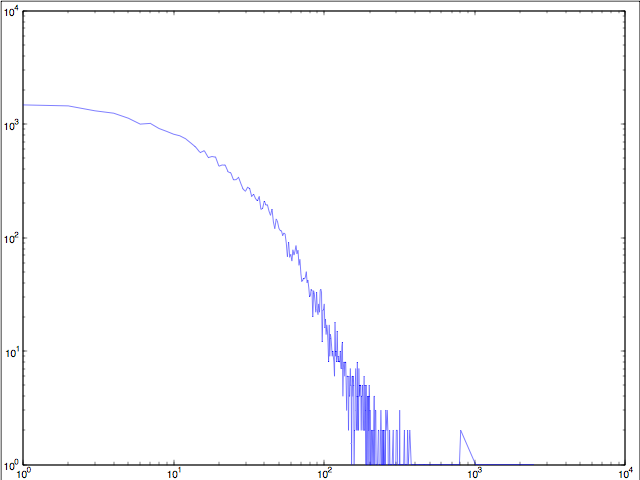
\includegraphics[width=.3\linewidth]{FIG/cit-HepTh-dd.png}}
\caption{Degree Distributions of cit-HepTh\label{fig:cit-HepTh_degree_dist}}
\end{figure}
\begin{figure}
\subfloat[In-Degree Distribution\label{fig:com-amazon.ungraph_indegree}]
  {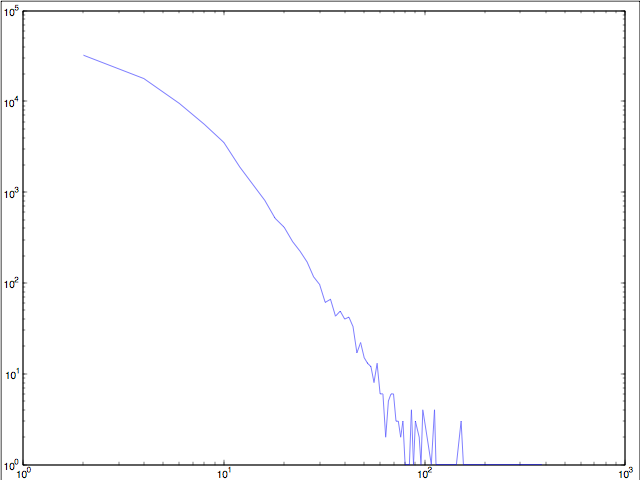
\includegraphics[width=.3\linewidth]{FIG/com-amazon.ungraph-indd.png}}\hfill
\subfloat[Out-Degree Distribution\label{fig:com-amazon.ungraph_outdegree}]
  {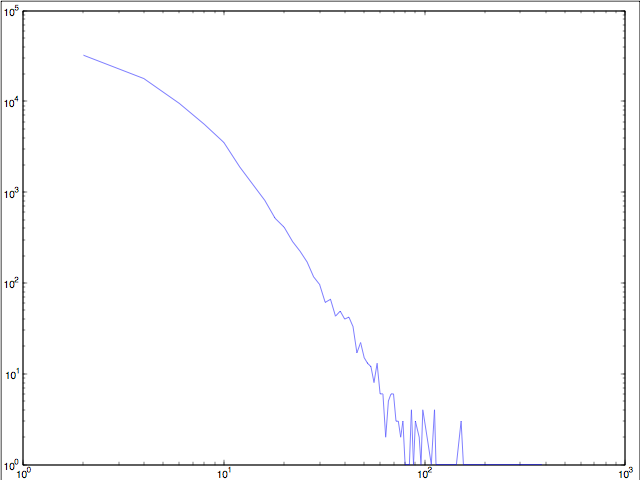
\includegraphics[width=.3\linewidth]{FIG/com-amazon.ungraph-outdd.png}}\hfill
\subfloat[Degree Distribution\label{fig:com-amazon.ungraph_degree}]
  {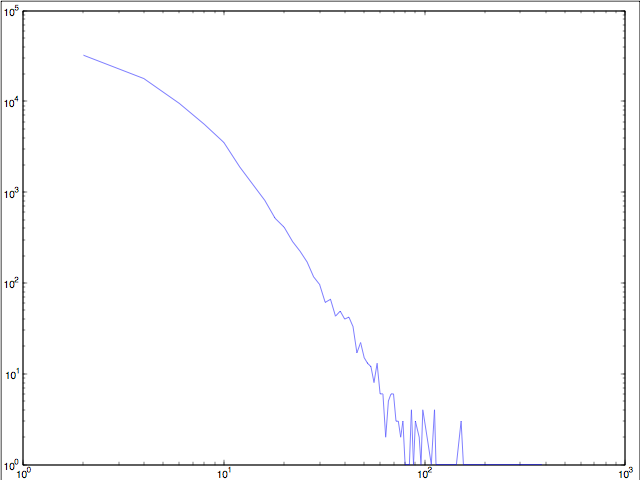
\includegraphics[width=.3\linewidth]{FIG/com-amazon.ungraph-dd.png}}
\caption{Degree Distributions of com-amazon.ungraph\label{fig:com-amazon.ungraph_degree_dist}}
\end{figure}
\begin{figure}
\subfloat[In-Degree Distribution\label{fig:com-dblp.ungraph_indegree}]
  {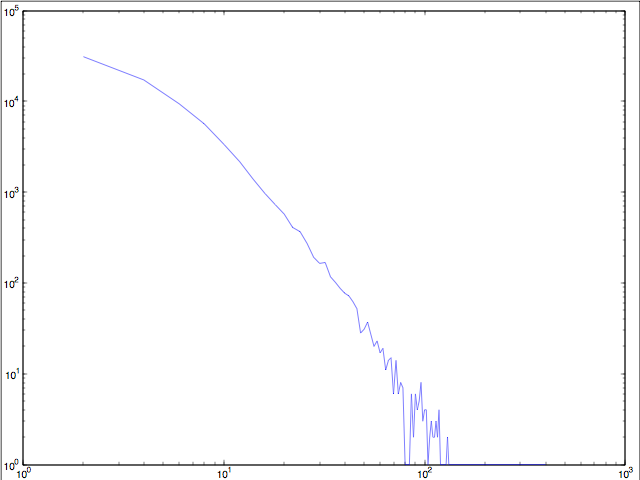
\includegraphics[width=.3\linewidth]{FIG/com-dblp.ungraph-indd.png}}\hfill
\subfloat[Out-Degree Distribution\label{fig:com-dblp.ungraph_outdegree}]
  {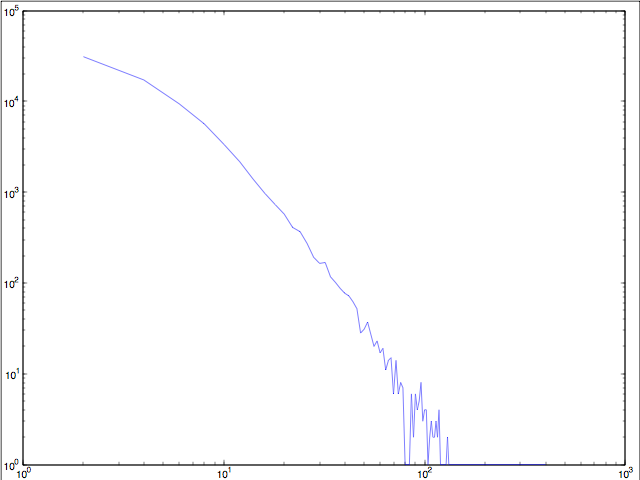
\includegraphics[width=.3\linewidth]{FIG/com-dblp.ungraph-outdd.png}}\hfill
\subfloat[Degree Distribution\label{fig:com-dblp.ungraph_degree}]
  {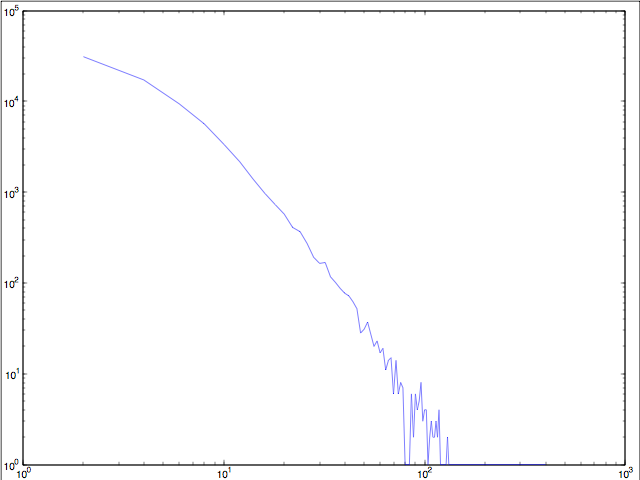
\includegraphics[width=.3\linewidth]{FIG/com-dblp.ungraph-dd.png}}
\caption{Degree Distributions of com-dblp.ungraph\label{fig:com-dblp.ungraph_degree_dist}}
\end{figure}
\begin{figure}
\subfloat[In-Degree Distribution\label{fig:email-Enron.ungraph_indegree}]
  {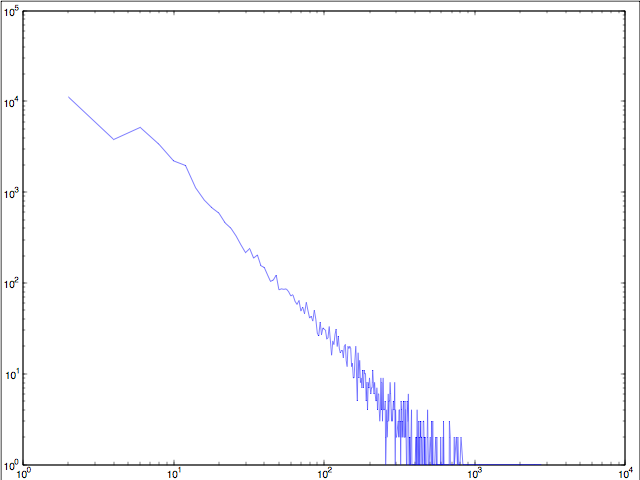
\includegraphics[width=.3\linewidth]{FIG/email-Enron.ungraph-indd.png}}\hfill
\subfloat[Out-Degree Distribution\label{fig:email-Enron.ungraph_outdegree}]
  {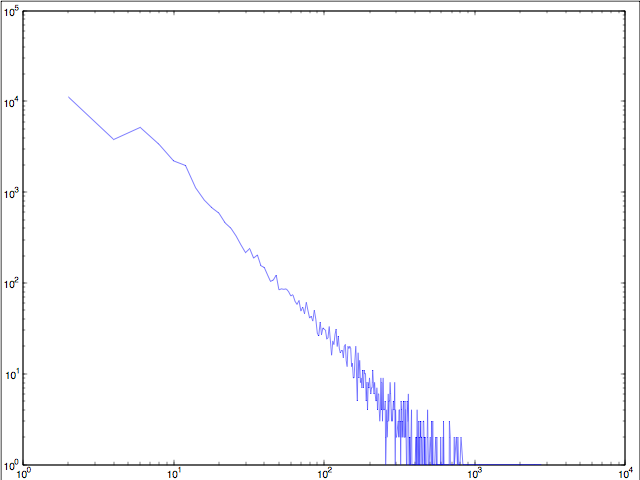
\includegraphics[width=.3\linewidth]{FIG/email-Enron.ungraph-outdd.png}}\hfill
\subfloat[Degree Distribution\label{fig:email-Enron.ungraph_degree}]
  {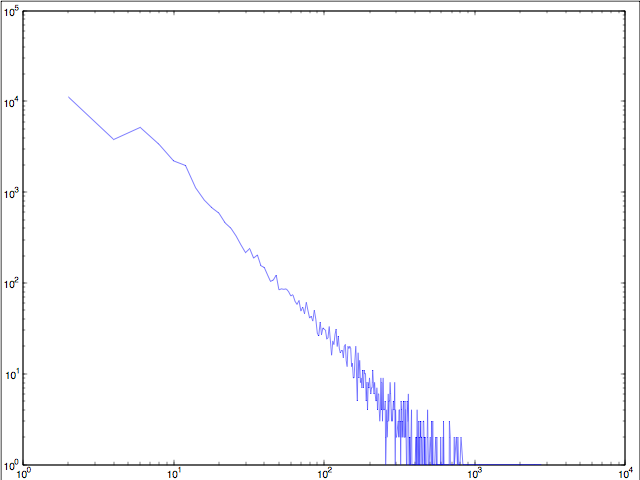
\includegraphics[width=.3\linewidth]{FIG/email-Enron.ungraph-dd.png}}
\caption{Degree Distributions of email-Enron.ungraph\label{fig:email-Enron.ungraph_degree_dist}}
\end{figure}
\begin{figure}
\subfloat[In-Degree Distribution\label{fig:email-EuAll_indegree}]
  {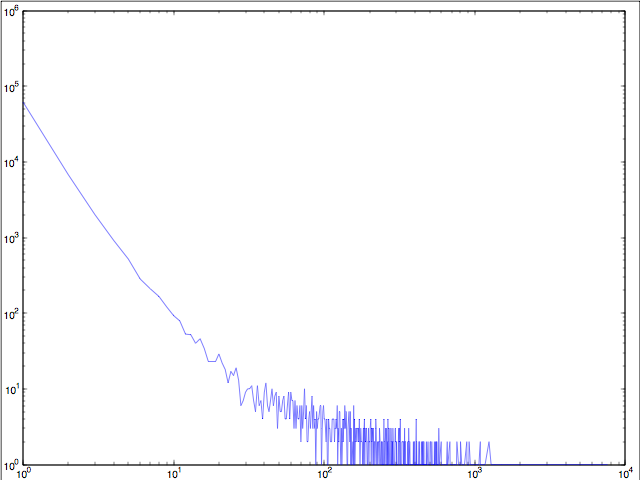
\includegraphics[width=.3\linewidth]{FIG/email-EuAll-indd.png}}\hfill
\subfloat[Out-Degree Distribution\label{fig:email-EuAll_outdegree}]
  {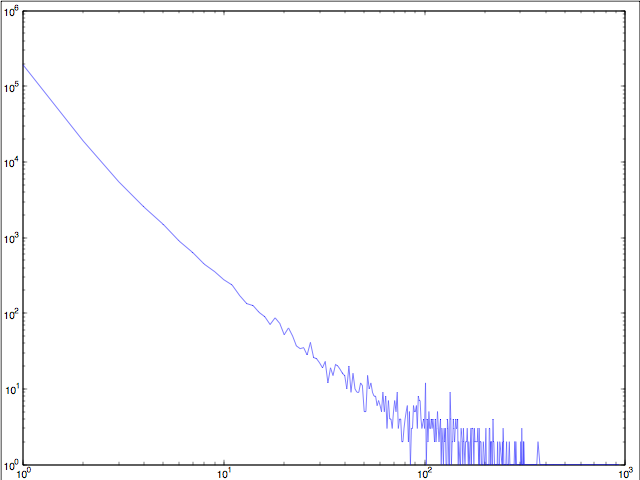
\includegraphics[width=.3\linewidth]{FIG/email-EuAll-outdd.png}}\hfill
\subfloat[Degree Distribution\label{fig:email-EuAll_degree}]
  {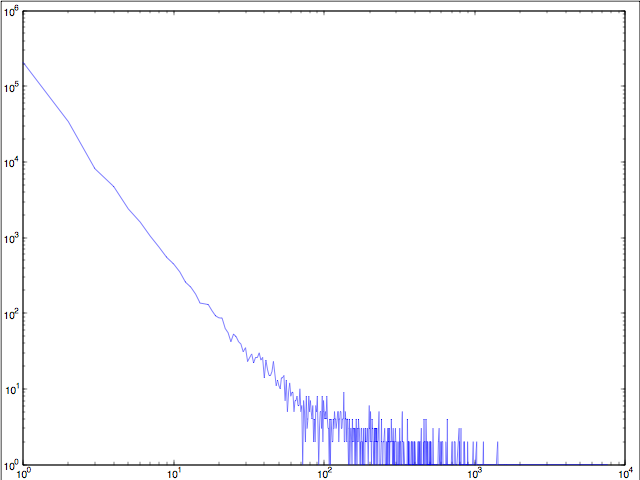
\includegraphics[width=.3\linewidth]{FIG/email-EuAll-dd.png}}
\caption{Degree Distributions of email-EuAll\label{fig:email-EuAll_degree_dist}}
\end{figure}
\begin{figure}
\subfloat[In-Degree Distribution\label{fig:p2p-Gnutella31_indegree}]
  {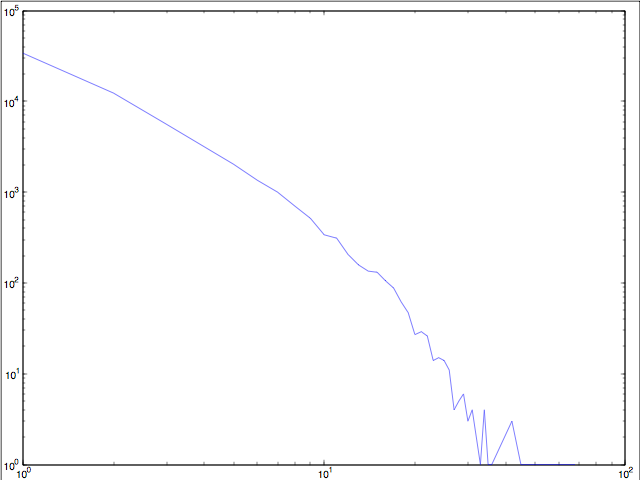
\includegraphics[width=.3\linewidth]{FIG/p2p-Gnutella31-indd.png}}\hfill
\subfloat[Out-Degree Distribution\label{fig:p2p-Gnutella31_outdegree}]
  {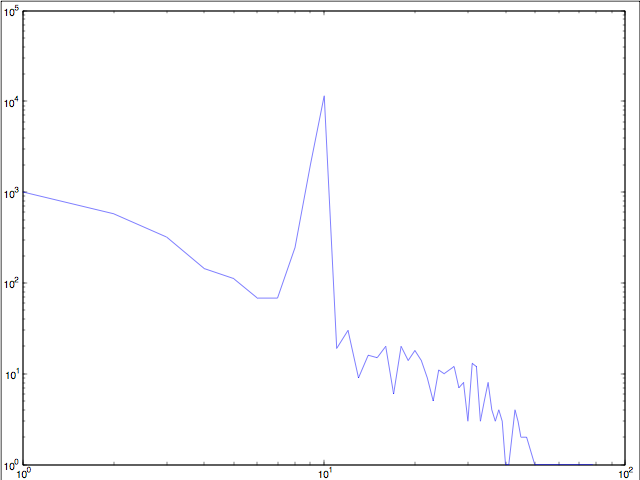
\includegraphics[width=.3\linewidth]{FIG/p2p-Gnutella31-outdd.png}}\hfill
\subfloat[Degree Distribution\label{fig:p2p-Gnutella31_degree}]
  {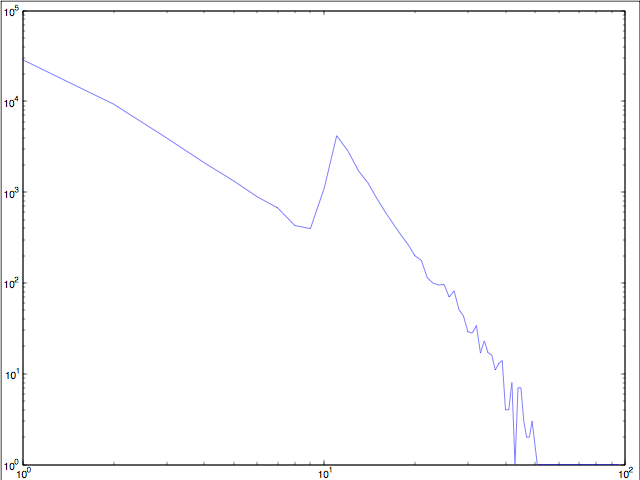
\includegraphics[width=.3\linewidth]{FIG/p2p-Gnutella31-dd.png}}
\caption{Degree Distributions of p2p-Gnutella31\label{fig:p2p-Gnutella31_degree_dist}}
\end{figure}
\begin{figure}
\label{deg_last}
\subfloat[In-Degree Distribution\label{fig:soc-Slashdot0811_indegree}]
  {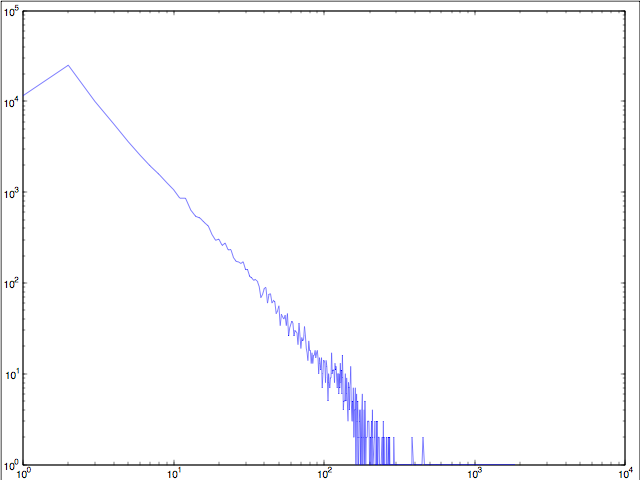
\includegraphics[width=.3\linewidth]{FIG/soc-Slashdot0811-indd.png}}\hfill
\subfloat[Out-Degree Distribution\label{fig:soc-Slashdot0811_outdegree}]
  {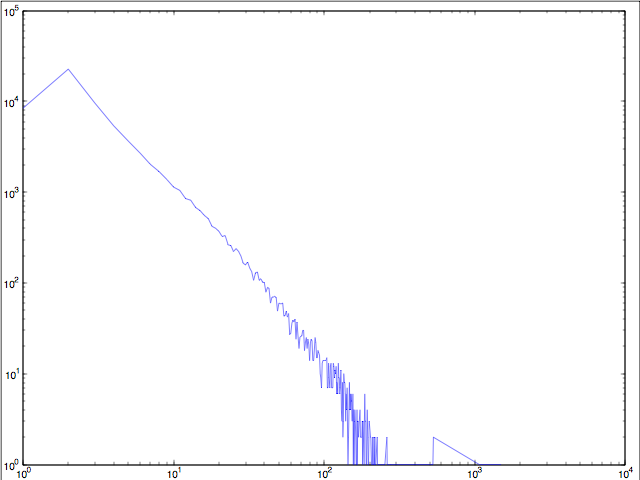
\includegraphics[width=.3\linewidth]{FIG/soc-Slashdot0811-outdd.png}}\hfill
\subfloat[Degree Distribution\label{fig:soc-Slashdot0811_degree}]
  {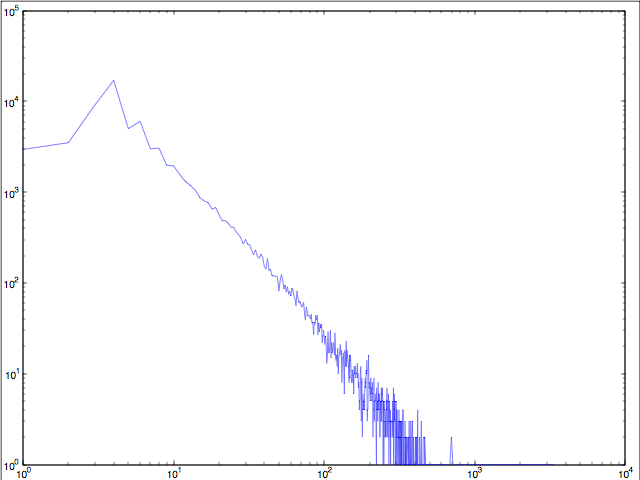
\includegraphics[width=.3\linewidth]{FIG/soc-Slashdot0811-dd.png}}
\caption{Degree Distributions of soc-Slashdot0811\label{fig:soc-Slashdot0811_degree_dist}}
\end{figure}

\subsubsection{Weakly Connected Component and Triangle count}

We find there are 2 highly connected graphs. p2p-Gnutella31 has 12 components and cit-HepPh has 61 components. This shows the nodes in these 2 graphs are mostly connected to each others.
On the other hand, email-EuAll has 15836 components. Although the maximun component size is huge, the connection between nodes are not strong in this graph.
\\
Triangle count shows that ca-AstroPh, cit-HepPh, email-Enron.ungraph are email-EuAll are densely connected. One interesting observation is that the p2p-Gnutella31 has very low triangle count, although the connected components shows that most nodes connect to each others in the graph. The may be caused by some very popular nodes. So that most nodes connect to these popular servers instead of connecting to each others.
\\
\\
\scalebox{0.8}{
\begin{tabular}{| l | c | c | c | c | c |} \hline
\textbf{Metrics} & \textbf{as-skitter} & \textbf{ca-AstroPh} & \textbf{cit-HepPh} & \textbf{cit-HepTh} & \textbf{com-amazon} \\ \hline
components & 310 & 290 & 61 & 143 & 1946 \\ \hline
max group & 69768 & 17926 & 34454 & 27465 & 47556 \\ \hline
triangle & 28389.34144 & 1061822.808 & 60696.51906 & 191035.2798 & 132.7590596 \\ \hline
\end{tabular}}\\
\\
\\
\scalebox{0.8}{
\begin{tabular}{| l | c | c | c | c | c |} \hline
\textbf{Metrics} & \textbf{com-dblp} & \textbf{email-Enron} & \textbf{email-EuAll} & \textbf{p2p-Gnutella31} & \textbf{soc-Slashdot0811} \\ \hline
components & 949 & 1065 & 15836 & 12 & 2091\\ \hline
max group & 67361 & 33696 & 224832 & 62561 & 72780\\ \hline
triangle & 786.338039 & 2059367.367 & 370075.0779 & 307.5803753 & 252186.8962\\ \hline
\end{tabular}}\

\subsubsection{PageRank}

The experiment result (Figure. \ref{fig:pagerank}) shows that the Pagerank value distribution in most of graphs follow power law.

\begin{figure}
\subfloat[as-skitter.75000\label{fig:as-skitter}]
  {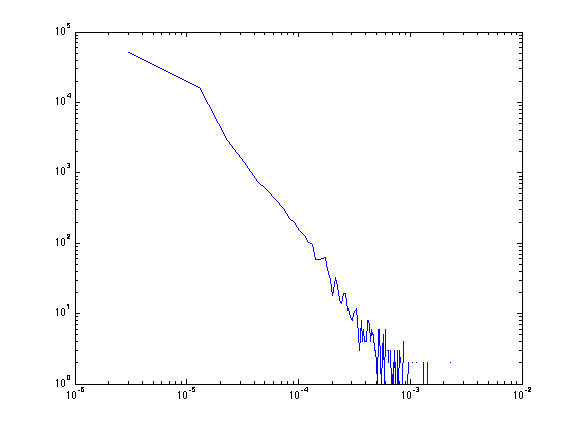
\includegraphics[width=.33\linewidth]{FIG/pagerank/as-skitter_75000.png}}\hfill
\subfloat[ca-AstroPh\label{fig:ca-AstroPh}]
  {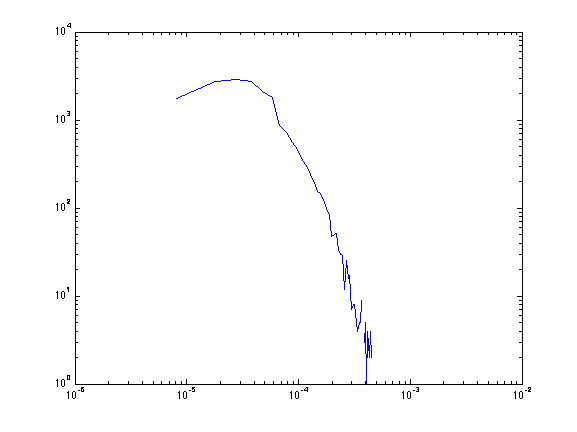
\includegraphics[width=.33\linewidth]{FIG/pagerank/ca-AstroPh.png}}\hfill
\subfloat[cit-HepPh\label{fig:cit-HepPh}]
  {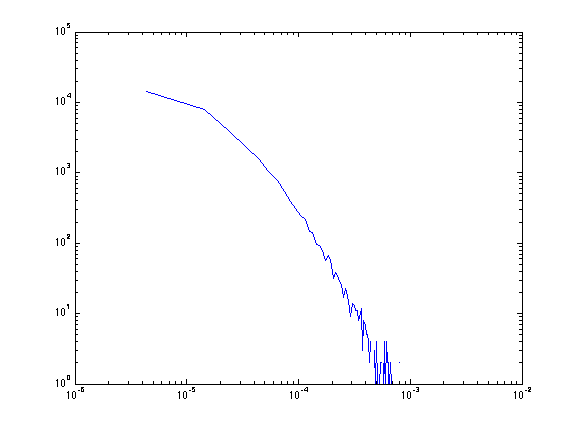
\includegraphics[width=.33\linewidth]{FIG/pagerank/cit-HepPh.png}} \hfill
\subfloat[cit-HepTh\label{fig:cit-HepTh}]
  {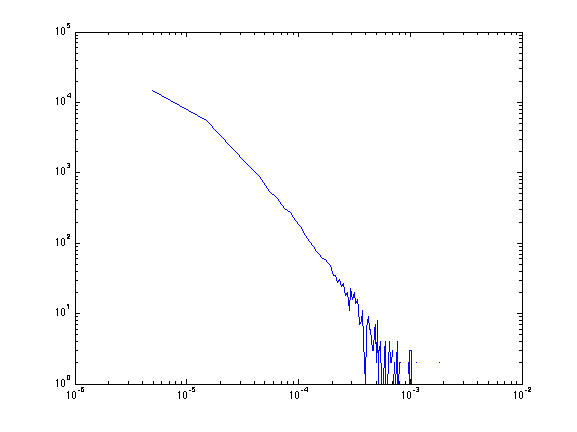
\includegraphics[width=.33\linewidth]{FIG/pagerank/cit-HepTh.png}}\hfill
\subfloat[com-amazon.ungraph-75000\label{fig:com-amazon.ungraph-75000}]
  {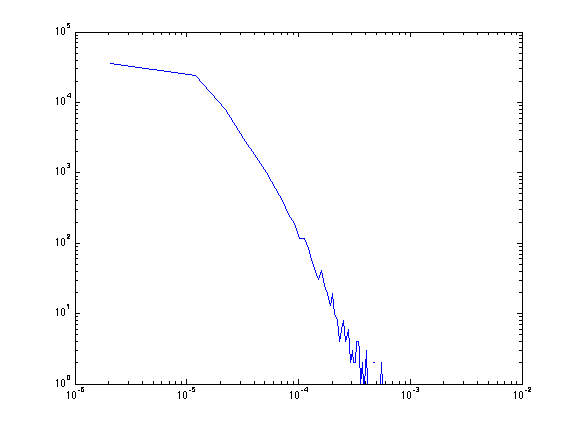
\includegraphics[width=.33\linewidth]{FIG/pagerank/com-amazon.ungraph-75000.png}}\hfill
\subfloat[com-dblp.ungraph-75000\label{fig:com-dblp.ungraph-75000}]
  {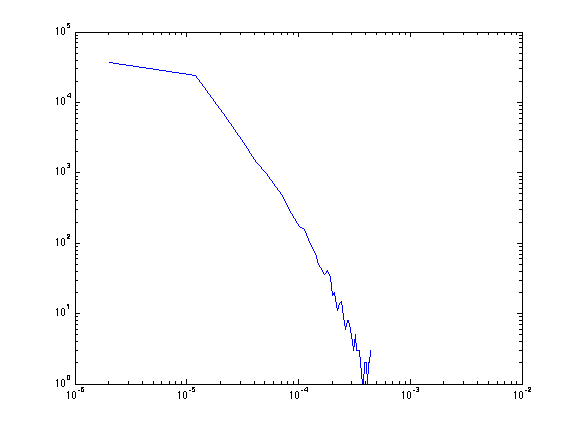
\includegraphics[width=.33\linewidth]{FIG/pagerank/com-dblp.ungraph-75000.png}} \hfill
 \subfloat[email-Enron.ungraph\label{fig:email-Enron.ungraph}]
  {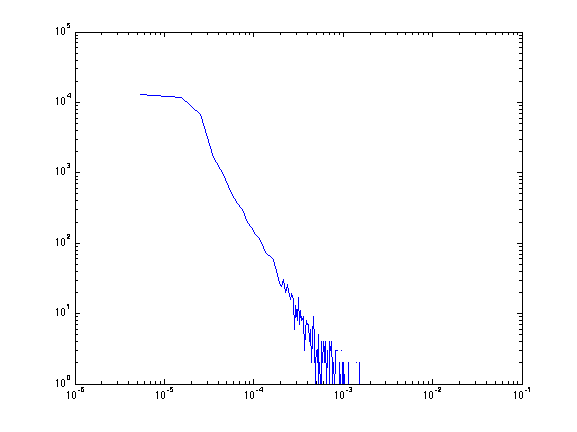
\includegraphics[width=.33\linewidth]{FIG/pagerank/email-Enron.ungraph.png}}\hfill
\subfloat[email-EuAll\label{fig:email-EuAll}]
  {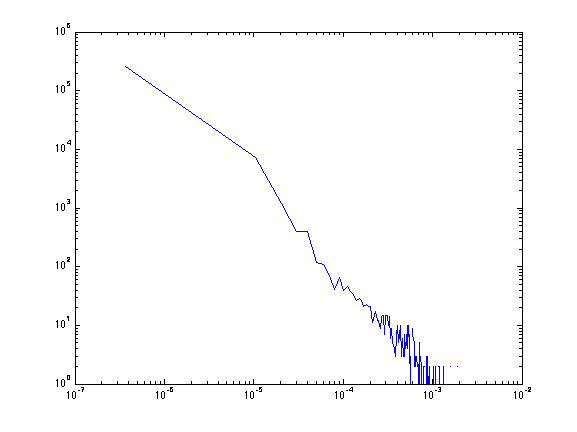
\includegraphics[width=.33\linewidth]{FIG/pagerank/email-EuAll.png}}\hfill
\subfloat[p2p-Gnutella31\label{fig:p2p-Gnutella31}]
  {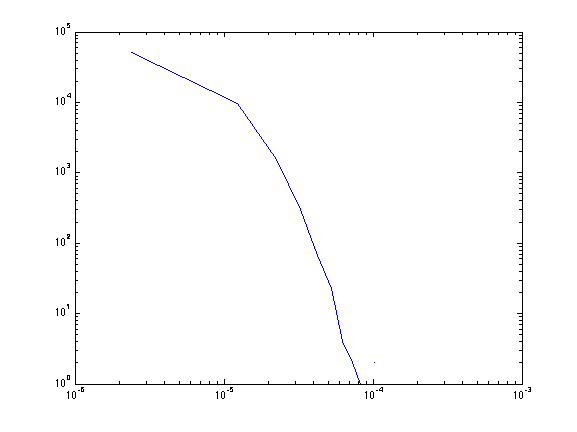
\includegraphics[width=.33\linewidth]{FIG/pagerank/p2p-Gnutella31.png}} \hfill
 \subfloat[soc-Slashdot0811-75000\label{fig:soc-Slashdot0811-75000}]
  {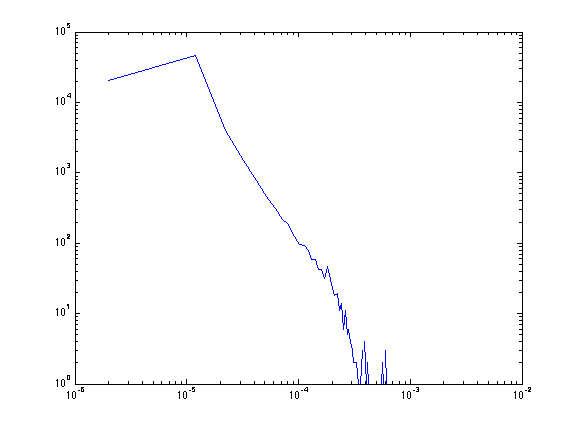
\includegraphics[width=.33\linewidth]{FIG/pagerank/soc-Slashdot0811-75000.png}} \hfill
\caption{Pagerank value Distributions of 10 graphs}
\label{fig:pagerank}
\end{figure}

\subsubsection{Eigenvalue computation (via Lanczos-SO and QR algorithms)}

\begin{center}
\scalebox{0.6}{
  \begin{tabular}{ |l | c | c | c | c | c | c |  }
    \hline
      & \textbf{cit-HepPh} & \textbf{com-amazon.ungraph-75000}  & \textbf{com-dblp.ungraph-75000}  & \textbf{email-Enron.ungraph}  & \textbf{soc-Slashdot0811-75000}  \\ \hline
First Eigenvalue & 71.24869215  & 12.46375985 & 18.08047143  & 232.0718265 & 124.3376448  \\ \hline
Second Eigenvalue & 15.78100055 & -10.49450063 & -9.989018866 & -52.74314639 & -74.23852603  \\ \hline
Third Eigenvalue & -11.28234916 & 2.528983265  & 3.950839681 & 16.07981363 & 3.277331459  \\ \hline
  \end{tabular}}
\end{center}

\begin{center}
\scalebox{0.6}{
  \begin{tabular}{ |l | c | c | c | c | c | c |  }
    \hline
      & \textbf{p2p-Gnutella31} & \textbf{ca-AstroPh} & \textbf{email-EuAll} & \textbf{cit-HepTh} & \textbf{as-skitter.75000}\\ \hline
First Eigenvalue & 12.26069439 & 182.7509283 & 134.5445114 & 108.0148181 & 182.7509283 \\ \hline
Second Eigenvalue & 2.714800955 & 64.42806942 & -59.94291686 & -48.59746457 & 64.42806942 \\ \hline
Third Eigenvalue & -2.60170164 & -0.449525922 & 6.537952019 & 9.103275079 & -0.449525922 \\ \hline
  \end{tabular}}
\end{center}

\subsubsection{K-core algorithm}

We set k = 5 and apply K-core algorithm on 10 graphs. The result shows that the graphs can be grouped into two types of graphs. Type I graphs, like soc-Slashdot0811-75000, p2p-Gnutella31, email-EuAll, email-Enron.ungraph, cit-HepTh, cit-HepPh, ca-AstroPh, have a giant 5-core with more than 7000 nodes, which means that type I graph is densely connected. Type II graphs, like com-dblp.ungraph-75000, com-amazon.ungraph-75000, and as-skitter.75000, do not have such a giant k-core. Instead, there are many small (size $<$ 500) 5-cores in type II graphs. It indicates that Type II graphs are not densely connected.

\begin{center}
\scalebox{0.6}{
  \begin{tabular}{ |c | c | c | c | c | c | c | c | c | c | c | c | c | c |  }
    \hline
         \multicolumn{2}{|c|}{soc-Slashdot0811-75000} & \multicolumn{2}{c|}{p2p-Gnutella31} & \multicolumn{2}{c|}{email-EuAll} & \multicolumn{2}{c|}{email-Enron.ungraph} & \multicolumn{2}{c|}{cit-HepTh} & \multicolumn{2}{c|}{cit-HepPh} & \multicolumn{2}{c|}{ca-AstroPh} \\ \hline
		size & frequency & size & frequency & size & frequency & size & frequency & size & frequency & size & frequency & size & frequency  \\ \hline
		26137  & 1 &16174  & 1 & 7030 & 1 & 6 & 6 & 21181 & 1 & 28593 & 1 & 6 & 2 \\ \hline
		& & & & & & 7 & 2 & & & & & 7 & 2 \\ \hline
		& & & & & & 8 & 3 & & & & & 8 & 1 \\ \hline
		& & & & & & 9 & 1 & & & & & 11 & 1 \\ \hline
		& & & & & & 12 & 1 & & & &  & 18 & 1 \\ \hline
		& & & & & & 15 & 1 & & & &  & 12236 & 1 \\ \hline
		& & & & & & 11538 & 1 & & & & &   &  \\ \hline
  \end{tabular}}
  \\5-core distribution in Type I graphs
\end{center}

\begin{center}
\scalebox{0.6}{
  \begin{tabular}{ |c | c | c | c | c | c |  }
    \hline
         \multicolumn{2}{|c|}{as-skitter.75000} & \multicolumn{2}{c|}{com-dblp.ungraph-75000} & \multicolumn{2}{c|}{com-amazon.ungraph-75000} \\ \hline
		size & frequency & size & frequency & size & frequency  \\ \hline
		14  & 1 & 6 & 9 & 6 & 1  \\ \hline
		181 & 1 & 7 & 3 & &   \\ \hline
		& & 8 & 3 & &  \\ \hline
		& & 9 & 1 & & \\ \hline
		& & 10 & 1 & & \\ \hline
		& & 13 & 1 & &  \\ \hline
		& & 15 & 1 & & \\ \hline
  \end{tabular}}
    \\5-core distribution in Type II graphs
\end{center}

